%---------------------------------- Optimization frame -------------------------------
\begin{frame}{Global optimization frame}
        \begin{block}{Diagram for the general principle}
            There are 2 importants steps : 
            \begin{itemize}
                \item Generate new solution : the optimization algorithm
                \item Evaluate the solution : application of the black-box function
            \end{itemize}
            
        \end{block}
            

            \begin{figure}
                \centering
                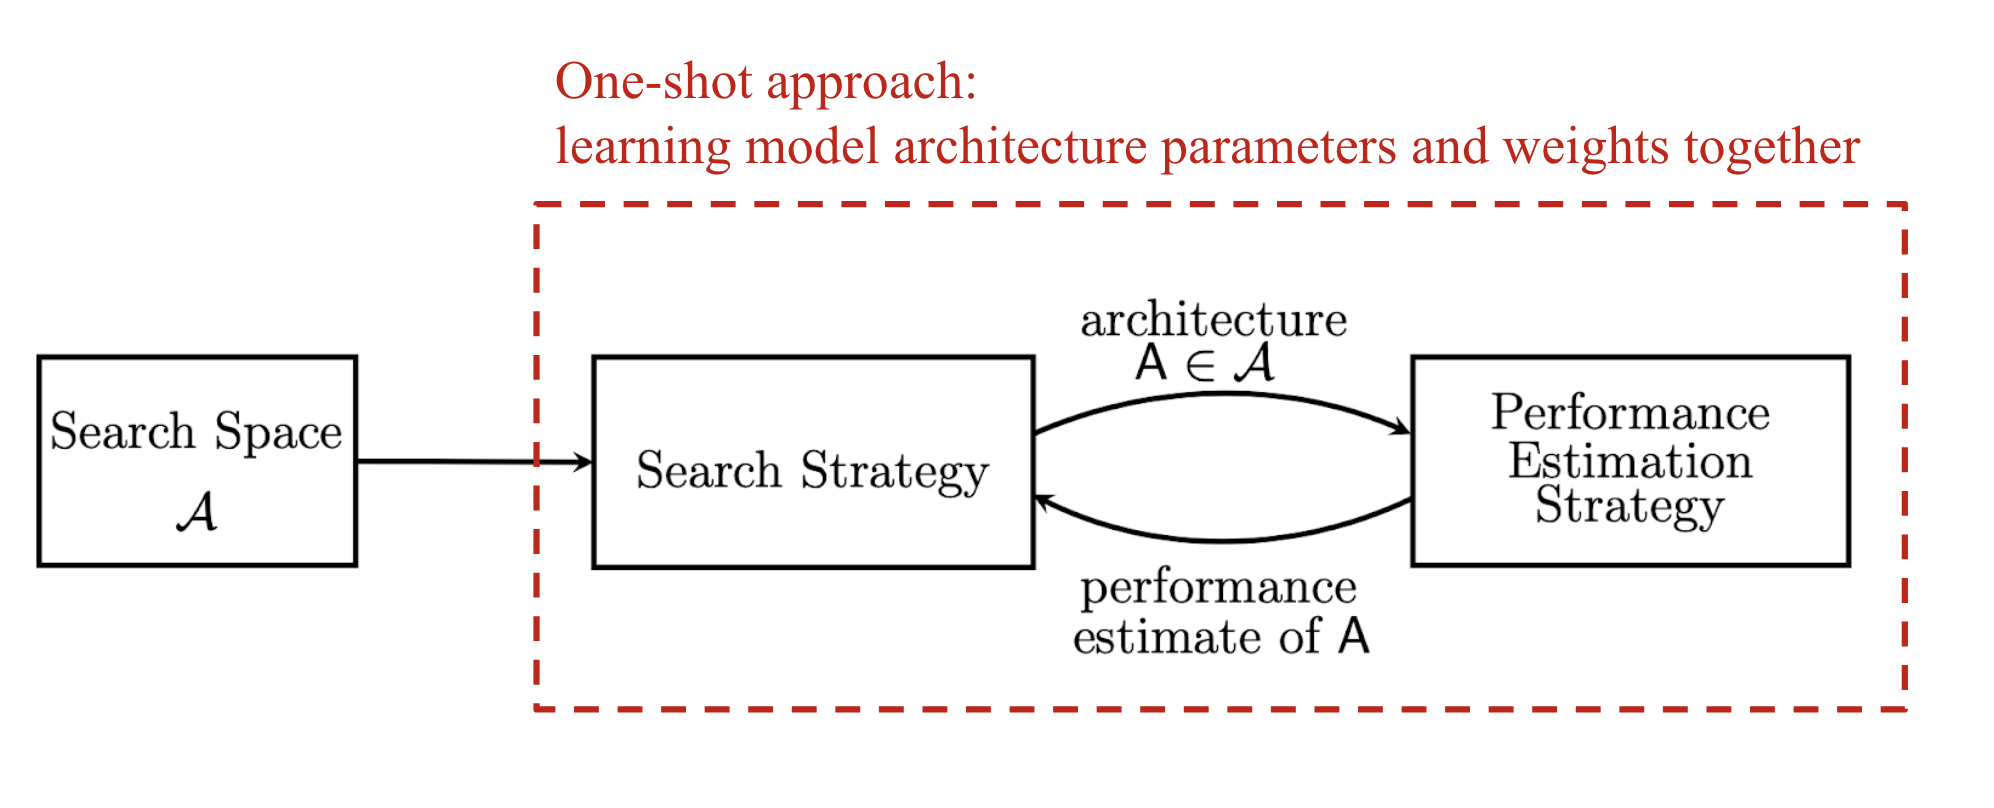
\includegraphics[width=0.5\linewidth]{imgs/NAS-high-level.png}
                \caption{Optimization frame}
            \end{figure}
    
\end{frame}

%---------------------------------- Optimization -------------------------------
\begin{frame}[allowframebreaks]{Optimization : generate the new solution}
    \begin{block}{Frameworks}
            The optimisation part is mostly done with Zellij, an open-source framework made for hyper-parameter optimization, composed of method from metaheuristics to fractals one, passing by bayesian based one.\\
            Some bayesian simulation are directly done with BoTorch.

        
    \end{block}

    \begin{block}{Used optimization algorithms}
        Present SOO, BO, BaMSOO
        
    \end{block}
\end{frame}



%---------------------------------- Evaluation Function -------------------------------
\begin{frame}[allowframebreaks]{Evaluate the solution}

    %---------------------------------- Training part -------------------------------
    
    \begin{columns}
        \begin{column}{0.45\textwidth}
            \begin{block}{Training frameworks}
                \begin{itemize}
                    \item Model : TinyLLama-1.B, lightweight LLama derived model. Imported with litgpt library. 
                    \item Training dataset : Alpaca\cite{alpaca}, a 52k entries Instructions Tuning datasets
                    \item Training loop : Pytorch Lightning framework, automating the training with class hooks
                \end{itemize}
            \end{block}
        \end{column}
        
        \begin{column}{0.55\textwidth}
            \begin{algorithm}[H]
            \begin{algorithmic}[1]
                \STATE HP = \textit{load\_hp()}
                \STATE data = \textit{LLMDataClass}()
                \STATE trainer = \textit{TrainerClass}(HP)
                \STATE model = \textit{LLMModelClass}(HP)
                \STATE trainer.\textit{fit}(model, data)
                \STATE \textit{merge\_lora\_weight}
                \STATE \textit{save}(model)
            \end{algorithmic}
            \caption{Training pseudocode}
            \label{alg:train}
            \end{algorithm}
        \end{column}
    \end{columns}
\framebreak

    %---------------------------------- Evaluate part -------------------------------

    \begin{columns}
        \begin{column}{0.35\textwidth}
            \begin{block}{Evaluation framework}
                \begin{itemize}
                    \item Evaluation framework: \texttt{lm\_eval} library
                    \item Benchmark dataset MMLU: imported from HuggingFace hub
                \end{itemize}
            \end{block}
        \end{column}
        
        \begin{column}{0.65\textwidth}
            \begin{algorithm}[H]
            \begin{algorithmic}[1]
                \STATE model = load\_model()
                \STATE eval\_dataset = datasets["mmlu"]
                \STATE predictions = model.predict(eval\_dataset.input)
                \STATE accuracy = \textit{compare}(predictions, eval\_dataset.output)
                \STATE return accuracy
            \end{algorithmic}
            \caption{Evaluate pseudocode}
            \label{alg:evaluate}
            \end{algorithm}
        \end{column}
    \end{columns}

    
\end{frame}